\usetikzlibrary{shapes.geometric, arrows}

\tikzstyle{startstop} = [rectangle,
minimum width=3cm, 
minimum height=1cm,
text centered, 
draw=black, 
fill=red!30]

\tikzstyle{io} = [trapezium, 
trapezium stretches=true, % A later addition
trapezium left angle=70, 
trapezium right angle=110, 
minimum width=3cm, 
minimum height=1cm, text centered, 
draw=black, fill=blue!30]

\tikzstyle{process} = [rectangle, 
minimum width=3cm, 
minimum height=1cm, 
text centered, 
text width=3cm, 
draw=black, 
fill=orange!30]

\tikzstyle{decision} = [diamond, 
minimum width=3cm, 
minimum height=1cm, 
text centered, 
draw=black, 
fill=green!30]
\tikzstyle{arrow} = [thick,->,>=stealth]

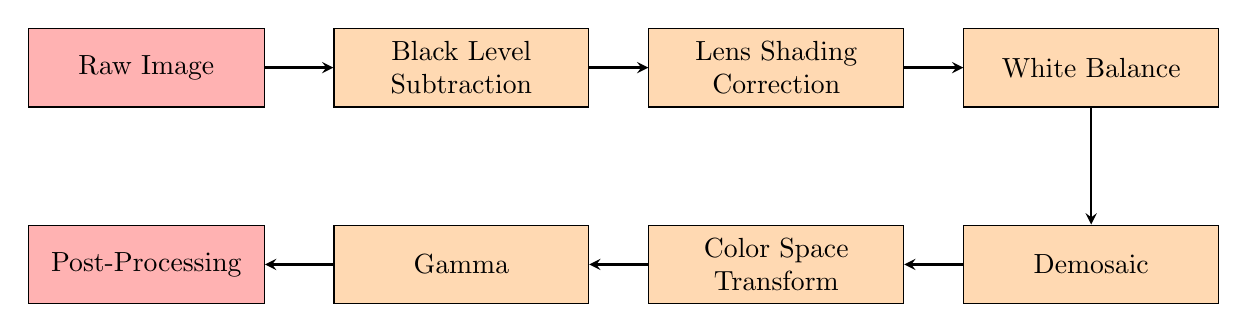
\begin{tikzpicture}[node distance=2cm]

\node (start) [startstop] {Raw Image};
\node (in1) [process, right of=start, xshift=2cm] {Black Level Subtraction};

\node (pro1) [process, right of=in1, xshift=2cm] {Lens Shading Correction};
\node (dec1) [process, right of=pro1, xshift=2cm] {White Balance};

\node (pro2a) [process, below of=dec1, yshift=-0.5cm] {Demosaic};

\node (pro2b) [process, left of=pro2a, xshift=-2cm] {Color Space Transform};
\node (pro2c) [process, left of=pro2b, xshift=-2cm] {Gamma};
\node (pro2d) [startstop, left of=pro2c, xshift=-2cm] {Post-Processing};



\draw [arrow] (start) -- (in1);
\draw [arrow] (in1) -- (pro1);
\draw [arrow] (pro1) -- (dec1);
\draw [arrow] (dec1) -- (pro2a);
\draw [arrow] (pro2a) -- (pro2b);
\draw [arrow] (pro2b) -- (pro2c);
\draw [arrow] (pro2c) -- (pro2d);

\end{tikzpicture}
